\documentclass[12pt, twoside, romanian]{report}
\usepackage{babel}
\usepackage{csquotes}
\usepackage{helvet}
\usepackage{lmodern}
\usepackage{graphicx}
\usepackage{fancyhdr}
\usepackage{geometry}
\usepackage{abstract}
\usepackage{titlesec}
\usepackage{enumitem}
\usepackage{multirow}
\usepackage{amsmath}
\usepackage[chapter]{minted}
\usepackage{xcolor}
\usepackage{hyperref}
\usepackage{cleveref}

\usepackage[style=ieee]{biblatex}

\addbibresource{bibliography.bib}

\definecolor{LightGray}{gray}{0.95}
\setminted[java] {
style=vs,
frame=single,
bgcolor=LightGray,
linenos
}

\renewcommand{\listingscaption}{Cod}
\renewcommand{\thelisting}{\thechapter.\arabic{listing}}
\crefname{listing}{Cod}{Cod}
\crefname{figure}{Figura}{Figura}

\newcommand{\university}{Universitatea Politehnica Timișoara}
\newcommand{\studyProgram}{Calculatoare și Tehnologia Informației}
\newcommand{\academicYear}{2022}
\newcommand{\firstName}{Prenume}
\newcommand{\lastName}{Nume}
\newcommand{\thesisTitle}{Titlul lucrării de finalizare a studiilor}
% Asist.(SL/Lect./Conf./Prof.)dr.ing.(arh./ec./chim.)
\newcommand{\coordinatorTitle}{dr.ing. }
\newcommand{\coordinatorFirstName}{Prenume}
\newcommand{\coordinatorLastName}{Nume}
\newcommand{\candidateName}{\firstName, \lastName}
\newcommand{\coordinator}{\coordinatorTitle \coordinatorFirstName, \coordinatorLastName}
% set document margins
\geometry{
 left=20mm,
 right=20mm,
 top=35mm,
 bottom=20mm,
 headheight=20mm,
 headsep=5mm
 }
 
 % set Helvetica as default font - it is the same as Arial
\renewcommand{\familydefault}{\sfdefault}
\linespread{1.15} 
\setlength{\parindent}{1.5cm}

% set chapter titles format
\titleformat
{\chapter}
[hang]
{\bfseries\fontsize{14pt}{18pt}\selectfont\MakeUppercase} % format
{\thechapter. }
{0cm}
{\centering}

\titlespacing
{\chapter}
{0cm}
{0pt}
{24pt}

% set section titles format
\titleformat
{\section}
[hang]
{\bfseries\fontsize{12pt}{16pt}\selectfont\MakeUppercase} % format
{\thesection}
{6.3mm}
{}

\titlespacing
{\section}
{0pt}
{12pt}
{12pt}

% set sub section titles format
\titleformat
{\subsection}
[hang]
{\fontsize{12pt}{16pt}\selectfont\MakeUppercase} % format
{\thesubsection}
{6.3mm}
{}

\titlespacing
{\subsection}
{0pt}
{12pt}
{12pt}
\fancypagestyle{titlepagestyle}{
    \fancyhf{}
    \fancyhead[L]{
        \fontsize{8}{9.2} \selectfont
        \studyProgram \\
        \textbf{\academicYear} \\
    }
    \fancyhead[R]{
\includegraphics{images/logo.png}}
    \fancyheadoffset[rh]{20mm}
    \renewcommand{\headrulewidth}{0pt}
    \renewcommand\footrulewidth{0pt}
}

\fancypagestyle{pagestyle}{
    \fancyhf{}
    \fancyhead[L]{
        \fontsize{8}{9.2} \selectfont
        \university, \studyProgram \\
        \academicYear \\
        \candidateName \\
        \thesisTitle \\
    }
    \fancyhead[R]{
\includegraphics{images/logo.png}}
    \fancyfoot[C]{- {\thepage} -}
    \fancyheadoffset[rh]{20mm}
    \renewcommand{\headrulewidth}{0pt}
    \renewcommand\footrulewidth{0pt}
}

\pagestyle{pagestyle}

\begin{document}

\begin{titlepage}
\thispagestyle{titlepagestyle}
    \begin{center}
        \vspace*{\fill}
        \textbf{\fontsize{20pt}{30pt} \selectfont \MakeUppercase{\thesisTitle}}
    \end{center}
    
    \vspace*{\fill}
     
            
    \textbf{\fontsize{14pt}{16pt} \selectfont Candidat: \candidateName}
    
    \vspace{14pt}
    
    \textbf{\fontsize{14pt}{16pt} \selectfont Coordonator științific: \coordinator}

    \begin{center}
        \vspace{50pt}
        \fontsize{14pt}{16pt} \selectfont Sesiunea: Iunie \academicYear 
    \end{center}
    

\end{titlepage}
\thispagestyle{pagestyle}

\begin{center}
    \textbf{\fontsize{20pt}{24pt} \selectfont Rezumat}
\end{center}

Rezumatul este destinat să informeze despre conținutul lucrării printr-o scurtă descriere a cercetării de maximum o pagină, a procedurilor/metodelor, precum și a rezultatelor sau concluziilor acesteia. Rezumatul în limba română devine obligatoriu pentru lucrările editate în alte limbi decât limba română și se va scrie cu caractere Arial de 12 pt. Acesta va începe la două rânduri lăsate libere după titlul "REZUMAT". Înainte de titlu se vor lăsa libere trei linii de 12 pt.

\vfill
\thispagestyle{pagestyle}

\begin{center}
    \textbf{\fontsize{20pt}{24pt} \selectfont Abstract}
\end{center}

The English abstract will be on the third page of the manuscriptand will present synthetically the paper work. The maximum length of the abstract is one page written with Arial characters, size 12 pt. The abstract text will begin after two blank lines (size 12pt.) from the “ABSTRACT” title. Before title there will be left three blank lines of 12pt size.

\vfill
\chapter{Introducere}
\thispagestyle{pagestyle}

Fiecare capitol trebuie să aibă o structură clară, va începe pe pagină nouă și va conține un titlu. Va fi urmat de două linii de 12 pt lăsate libere.

\section{Informații generale}

Fiecare secțiune a unui capitol (ex. 1.1 INFORMAȚII GENERALE) va fi poziționat la un rând liber sub text și va avea un rând liber de12 pt deasupra textului. 

Textul lucrării va fi aliniat uniform (justify). Este de preferat ca textul să fie verificat pentru eventualele erori în limba de editare cu ajutorul facilității de verificare a ortografiei (speller) din programul word. Este recomandat ca lucrarea de finalizare a studiilor să nu depășească 100 de pagini, inclusiv anexele.

Reguli aplicate pentru textul lucrării:
\begin{enumerate}[leftmargin=2cm,topsep=1.15pt,itemsep=1.15pt,partopsep=1.15pt,parsep=1.15pt,label=\alph*.]
   \item Marginile paginii – se vor utiliza următoarele valori pentru marginile paginii
   \begin{itemize}[topsep=1.15pt,itemsep=1.15pt,partopsep=1.15pt,parsep=1.15pt]
     \item interior: 2 cm 
     \item exterior: 2 cm 
     \item sus: 2,5 cm (inclusiv header)
     \item jos: 2 cm
   \end{itemize}
   \item Spațiere între rânduri - textul va respecta o spațiere între rânduri de 1,15 linii
   \item Alinierea textului în cadrul paragrafelor - textul din cadrul paragrafelor normale va fi aliniat între marginile din stânga şi dreapta. Primul rând al fiecărui paragraf va avea o aliniere de 1,5 cm. Excepție fac titlurile capitolelor, care vor fi aliniate la stânga, precum și etichetele tabelelor și ale figurilor (conform explicațiilor de mai jos)
   \item Font – fontul utilizat pentru redactare va fi Arial, cu dimensiunea de 12 puncte, utilizând diacriticele specifice limbii în care este redactată lucrarea (ex: ă, ş, ţ, î, â - pentru limba română);
   \item Numerotarea paginilor - numerotarea paginilor se face începând cu pagina de titlu, până la ultima pagină a lucrării, dar numărul paginii apare doar începând cu Introducerea. Numărul de pagină se inserează în subsolul paginii, centrat.
   \item Antetul paginii – apare începând cu introducerea și va conține pe rânduri succesive un text cu înălțimea de 8, aliniat la stânga: (i) textul Universitatea Politehnica Timișoara ; (ii) denumirea programului de studii și anul susținerii ; (iii) numele candidatului (în stânga) și titlul lucrării. În partea dreaptă a antetului poate fi integrată sigla UPT;
\end{enumerate}
\chapter{Conținut}
\thispagestyle{pagestyle}

\section{Figuri și fotografii}

Figurile (incluzând imagini, grafice, capturi de ecran) se numerotează în ordinea apariției în lucrare. Alternativ, figurile pot fi numerotate în ordine în fiecare capitol, integrând în numerotare și numărul capitolului. Fiecare figură are număr și titlu, care se menționează sub figură, centrat. Dacă este cazul, sursa figurii se indică între paranteze după titlul figurii. Toate figurile şi fotografiile prezentate în lucrare trebuie să fie referite în textul lucrării, trebuie să fie numerotate şi însoţite de titlul figurii.

Se va lăsa câte o linie liberă (Arial 12 pt) între figură şi text. Figurile vor fi centrate pe pagină.

\begin{figure}[h]
\centering
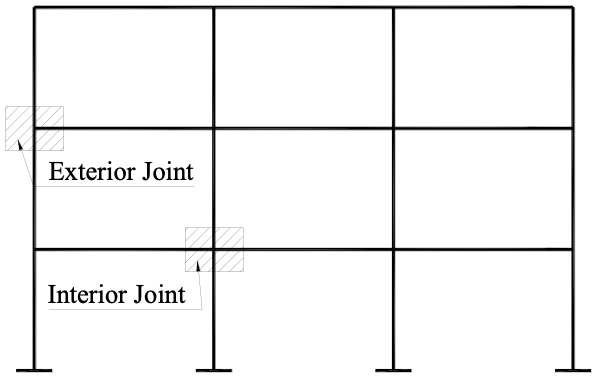
\includegraphics{images/Picture 1.png}
\caption{Exemplu de figură (sursa: Buletinul ştiinţific al UPT seria construcţii-arhitectură nr.2 /2010)}
\label{fig:fig2.1}
\end{figure}

\section{Tabele}

Tabele – tabelele se numerotează în ordinea apariției în lucrare. Alternativ, tabelele pot fi numerotate în ordine în fiecare capitol, integrând în numerotare și numărul capitolului. Fiecare tabel are număr și titlu, care se menționează deasupra tabelului, aliniat centrat. Dacă este cazul, sursa datelor se precizează între paranteze după titlul tabelului.

Toate tabelele prezentate în lucrare trebuie să fie referite în textul lucrării, trebuie să fie numerotate şi însoţite de un titlu (vezi exemplul de mai jos). Dacă se utilizează figuri copiate atunci se va indica sursa fotografiei în paranteză. Pe cât posibil, în tabel se va păstra fontul uzual (arial 12 pt) dar sunt acceptate şi modalităţi de a scoate în evidenţă rezultatele importante (bold, italic etc.)

Se va lăsa câte o linie liberă (arial 12 pt) între text şi tabel. Tabelele vor fi centrate pe pagină.

\begin{table}[ht]
\centering
\caption{Exemplu de tabel}
\label{table:table1}
\begin{tabular}{ |p{2.9cm}|p{2.45cm}|p{4cm}|p{2.45cm}|p{4cm}|  }
 \hline
  &  \multicolumn{2}{|c|}{Yield stress, fy [N/mm2]} & \multicolumn{2}{|c|}{Tensile strength, fu [N/mm2]} \\
 \hline
 Element & Mill certificate & Coupon tests & Mill certificate & Coupon tests \\
 \hline
 Beam IPE360 & 285.0 & 329.8 flange 348.4 web & 427.0 & 463.2 flange 464.0 web \\
 \hline
 Column HEB300 & 311.3 & 313.0 flange 341.8 web	& 446.0	& 449.8 flange 464.4 web \\
 \hline
 End plate & 281.0 & 248.3 & 424.7 & 416.0 \\
 \hline
 Cover plate & 296.0 & 273.2 & 443.0 & 436.7 \\
 \hline
\end{tabular}
\end{table}

\section{Formule}

Formulele utilizate în text se vor numerota în ordinea apariției în lucrare. Alternativ, formulele pot fi numerotate în ordine în fiecare capitol, integrând în numerotare și numărul capitolului. Numerotarea formulelor se face în paranteze rotunde. Se va lăsa câte o linie liberă (arial 12 pt) între text şi formulă. Formulele vor fi aliniate la dreapta.

\begin{equation}
A=\pi*r^2
\end{equation}
\chapter{Concluzii}
\thispagestyle{pagestyle}

Lucrarea se va încheia cu un capitol de concluzii. Acesta va conţine principalele rezultate ale lucrării şi implicaţiile practice ale acestora. În cazul proiectelor de diplomă, se vor menționa principalele date sintetice obținute din procesul de proiectare.

\section{Bibliografie}
La sfârşitul lucrării va fi dată o listă de referinţe pentru textele ştiinţifice consultate pe parcursul realizării lucrării. Vor fi trecute toate sursele, inclusiv cele de pe internet. Acestea vor fi referite în text şi trecute în lista de referinţe în ordine alfabetică, după exemplele de mai jos. 

Bibliografia trebuie să cuprindă toate titlurile din literatura de specialitate care au servit ca bază de documentare, respectiv autorii care au fost citați în text, la toate capitolele lucrării. 

În cadrul Facultății de Automatică și Calculatoare se cere folosirea stilului de citare IEEE (detalii IEEE Citation Guidelines2.doc (ieee-dataport.org)), folosit cu precădere în publicațiile științifice din domeniul IT. Cele trei părți importante ale referinței sunt:
\begin{enumerate}[leftmargin=2cm,topsep=1.15pt,itemsep=1.15pt,partopsep=1.15pt,parsep=1.15pt,label=\alph*.]
   \item Numele autorului indicat ca prima inițială a prenumelui, apoi numele complet.
   \item Titlul articolului, brevetul, lucrarea de conferință etc., între ghilimele.
   \item Titlul revistei sau cărții cu caractere cursive
Modul de redactare a referinței depinde de tipul publicației, vă rugăm să urmăriți cu atenție indicațiile de la link-ul de mai sus.
\end{enumerate}
	 
Fiecare citare trebuie notă în text prin utilizarea unor numere secvențiale simple. Un număr cuprins între paranteze drepte, plasat în textul raportului, indică referința specifică. Citările sunt numerotate în ordinea în care apar. Odată ce o sursă a fost citată, același număr este folosit în toate referințele ulterioare din text. Nu se face distincție între sursele electronice și cele tipărite, cu excepția detaliilor referințelor citate.

Fiecare număr de referință trebuie să fie cuprins între paranteze drepte pe aceeași linie cu textul, înaintea oricărei semne de punctuație, cu un spațiu înaintea parantezei.

Exemple:
\begin{enumerate}[leftmargin=2cm,topsep=1.15pt,itemsep=1.15pt,partopsep=1.15pt,parsep=1.15pt,label=\alph*.]
   \item ". . .finalul cercetării mele [13]."
   \item "Teoria a fost prezentată pentru prima dată în 1987 [1]."
\end{enumerate}

Lista de referințe din bibliografie este compusă din toate sursele folosite pentru documentarea lucrării și se realizează în ordinea numerică a citării în text și nu în ordine alfabetică a autorilor.

Preluarea identică a unei fraze sau paragraf va fi citată prin indicarea inclusiv a paginii din sursa utilizată, dar și prin ghilimele şi forma italică a literelor; pentru sursele preluate de pe internet, vor fi notate adresele de pagină web; în lista bibliografică finală lucrările se trec în ordinea alfabetică a numelor autorilor. La lucrările colective, regula referitoare la ordinea alfabetică este valabilă pentru primul autor. 

Dacă se citează site-uri web, reviste sau articole, înainte de acestea se vor trece trei asteriscuri, informații referitoare la volum, număr, pagini consultate, adresa web exactă a articolului respectiv, data vizitării site-ului și a descărcării materialului, data accesării. Adresele de pagini web se regăsesc la finalul listei.

Sursele bibliografice la care nu se poate menționa autorul se vor specifica astfel: "***" urmat de denumirea articolului și/sau a cărții, editura și locul apariției (pentru cărți), volumul, numărul acestuia, prima și ultima pagină a lucrării citate, anul apariției. 

*** https://ro.wikipedia.org/wiki/Motor accesare februarie 2022

Exemplu citare: Einstein \cite{einstein}

\section{Declarația de autenticitate}
Ultima pagină a lucrării de licență/diplomă/disertație trebuie să conțină "Declarația de originalitate a lucrării de finalizare a studiilor", completată olograf, în conformitate cu cerinţele UPT. Declaraţia se descarcă de pe adresa de web: 

\url{http://www.upt.ro/img/files/Regulamente_UPT/2020/Declaratie_de_autenticitate_UPT_2020.pdf}

% Look for building the .bib file on Overleaf documentation

\printbibliography
\thispagestyle{pagestyle}

\end{document}